\documentclass[10pt]{article}
\usepackage{fullpage}
\usepackage{enumitem}
\usepackage{amsmath}
\usepackage{amssymb}
\usepackage{graphicx}
\usepackage[T1]{fontenc}
\usepackage{lipsum}
\usepackage{listings}
\usepackage{float}
\usepackage{scrextend}
\usepackage{hyperref}
\usepackage{algorithmicx}
\usepackage{algpseudocode}
\usepackage{tikz}
\usepackage{pgfplots}
\usetikzlibrary{arrows,
                backgrounds,
                fit,
                positioning,
                quotes,
                shapes,
                pgfplots.colorbrewer,
}
                
\usepackage{xcolor}
\usepackage{wrapfig}


\pgfplotsset{
    cycle from colormap manual style/.style={
        x=3cm,y=10pt,ytick=\empty,
        stack plots=y,
        every axis plot/.style={line width=2pt},
    },
}

%\pagecolor[rgb]{0,0,0}
%\pagecolor[rgb]{0.0549,0.0667,0.0862}

\iffalse
\pagecolor[rgb]{0.1269, 0.1369, 0.1469}
\color[rgb]{1,1,1}

\fi

\newenvironment{subs}
  {\adjustwidth{3em}{0pt}}
  {\endadjustwidth}

\title{\vspace{-1cm} \Huge Project 1 \\ \LARGE CmpE 300, Analysis of Algorithms, Fall 2022 }
\author{
    Bahadır Gezer - 2020400039 \\
    Muhammet Batuhan Ilhan - 2019400xxx \\
}
\date{November 2022}

\begin{document}
\maketitle
  
\tableofcontents

\newpage
\section{Theoretical Analysis}

\begin{quote}
\begin{algorithmic}[1]
\Require $n = 2^{k}-1$, $k \in \mathbb{Z}^{+}$
\Require $arr[i] \in \{0,1,2\}$, $0 \leq i \leq n-1$
\State $\textbf{Input: } arr[0:n-1]$ 
\State $\textbf{Output: } arr2[0:4]$ 
\State $\textbf{function }Example(arr[0:n-1])$
\State 
\State $arr2 \gets [0,0,0,0,0]$
\For {$i \gets 0 \textbf{ to } n-1$}
    \If{$arr[i] = 0$}
        \For {$t1 \gets i \textbf{ to } n-1$}
            \State $p1 \gets t1^{1/2}$
            \State $x1 \gets n + 1$
            \While{$x1 \geq 1$}
                \State $x1 \gets \lfloor x1 / 2 \rfloor$
                \State $arr2[i \bmod 5] \gets arr2[i \bmod 5] + 1$
            \EndWhile
        \EndFor
    \ElsIf{$arr[i] = 1$}
        \For{$t2 \gets n \textbf{ down to } 1$}
            \For{$p2 \gets 1 \textbf{ to } n$}
                \State $x2 \gets n + 1$
                \While{$x2 > 0$}
                    \State $x2 \gets \lfloor x2 / 2 \rfloor$
                    \State $arr2[i \bmod 5] \gets arr2[i \bmod 5] + 1$
                \EndWhile
            \EndFor
        \EndFor
    \ElsIf{$arr[i] = 2$}
        \For{$t3 \gets 1 \textbf{ to } n$}
            \State $x3 \gets t3 + 1$
            \For{$p3 \gets 0 \textbf{ to } t3^{2} - 1$}
                \State $arr2[i \bmod 5] \gets arr2[i \bmod 5] + 1$
            \EndFor
        \EndFor
    \EndIf
\EndFor
\State $\textbf{end}$
\end{algorithmic}
\end{quote}

\begin{description}
   \item[for loop 1 - line 6:] This loop will iterate \textbf{from} $0$ \textbf{to}  $\mathbf{n-1}$. Which is a total of $\mathbf{n}$ iterations. 
   
   \item[for loop 2 - line 8:] This loop will iterate \textbf{from} $\mathbf{i}$ \textbf{to}  $\mathbf{n-1}$. Which is a total of $\mathbf{n-i}$ iterations. 

    \begin{align*}
    i &= 0 \text{\hspace{0.5cm}loop iterates n times} \\
    i &= 1 \text{\hspace{0.5cm}loop iterates n - 1 times}\\
    i &= 2 \text{\hspace{0.5cm}loop iterates n - 2 times}\\
    &\vdots \\
    i &= n - 1 \text{\hspace{0.5cm}loop iterates 1 time} \\
    \end{align*}

    Therefore, this loop iterates \mathbf{\frac{n*(n+1)}{2}} times. In this calculation we take the for loop 1 into account.

   \item[while loop 1 - line 11:] This loop will iterate \textbf{from} $\mathbf{n+1}$ \textbf{to} $\mathbf{1}$ by halving at each iteration. For the sake of simplicity, lets consider $\mathbf{n+1}$ as $\mathbf{2^{z}}$ where $\mathbf{z}$ is some positive integer. It will be generalized using interpolation later.
   \begin{enumerate}[leftmargin=3cm]
       \item[\textit{\textbf{Iteration 1 -}}] ${k = 2^{z}}$
       \item[\textit{\textbf{Iteration 2 -}}] ${k = 2^{z-1}}$
       \item[\textit{\textbf{Iteration 3 -}}] ${k = 2^{z-2}}$
       \item[]\hspace{-1.5cm}\textbf{\vdots}\hspace{2cm}\textbf{\vdots}
       \item[\textit{\textbf{Iteration m -}}] ${k = 2^{z-m-1} = 1}$
   \end{enumerate}
  As seen above, the loop will iterate $\mathbf{m}$ times. Solving the equation $\mathbf{2^{z-m-1} = 1}$ for $\mathbf{m}$ we get $\mathbf{m = z - 1}$. Substituting $\mathbf{z = log_2(n+1)}$ into the equation we get $\mathbf{m = log_2(n+1) - 1}$. Thus, the loop will have $\mathbf{log_2(n+1) - 1}$ iterations. The last iteration does not count, because of the termination statement of the while loop, so the real number of iterations is $\mathbf{log_2(n+1) - 2}$.

    \item[for loop 3 - line 17:] This loop will iterate \textbf{from} $\mathbf{n}$ \textbf{to}  $\mathbf{1}$. The loop is not interrupted mid iteration. Thus the total number of iterations come out to be $\mathbf{n}$. 

    \item[for loop 4 - line 18:] This loop will iterate \textbf{from} $\mathbf{1}$ \textbf{to}  $\mathbf{n}$. The loop is not interrupted mid iteration. Thus the total number of iterations come out to be $\mathbf{n}$. 

   \item[while loop 2 - line 20:] This loop will iterate \textbf{from} $\mathbf{n+1}$ \textbf{to} $\mathbf{1}$ by halving at each iteration. For the sake of simplicity, lets consider $\mathbf{n+1}$ as $\mathbf{2^{z}}$ where $\mathbf{z}$ is some positive integer. 
   \begin{enumerate}[leftmargin=3cm]
       \item[\textit{\textbf{Iteration 1 -}}] ${k = 2^{z}}$
       \item[\textit{\textbf{Iteration 2 -}}] ${k = 2^{z-1}}$
       \item[\textit{\textbf{Iteration 3 -}}] ${k = 2^{z-2}}$
       \item[]\hspace{-1.5cm}\textbf{\vdots}\hspace{2cm}\textbf{\vdots}
       \item[\textit{\textbf{Iteration m -}}] ${k = 2^{z-m-1} = 1}$
   \end{enumerate}
 As seen above, the loop will iterate $\mathbf{m}$ times. Solving the equation $\mathbf{2^{z-m-1} = 1}$ for $\mathbf{m}$ we get $\mathbf{m = z - 1}$. Substituting $\mathbf{z = log_2(n+1)}$ into the equation we get $\mathbf{m = log_2(n+1) - 1}$. Thus, the loop will have $\mathbf{log_2(n+1) - 1}$ iterations. \par


\item[for loop 5 - line 27:] This loop will iterate \textbf{from} $\mathbf{1}$ \textbf{to} $\mathbf{n}$. The loop is not interrupted mid iteration. Thus the total number of iterations come out to be $\mathbf{n}$. 

\item[for loop 6 - line 29:] This loop will iterate \textbf{from} $\mathbf{0}$ \textbf{to} $\mathbf{t3^2-1}$. 
    \begin{align*}
    t3 &= 0 \text{\hspace{0.5cm}loop iterates $\mathbf{0^{2}}$ times} \\
    t3 &= 1 \text{\hspace{0.5cm}loop iterates $\mathbf{1^{2}}$ times}\\
    t3 &= 2 \text{\hspace{0.5cm}loop iterates  $\mathbf{2^{2}}$ times}\\
    &\vdots \\
    t3 &= n - 1 \text{\hspace{0.5cm}loop iterates $\mathbf{(n-1)^{2}}$ time} \\
    \end{align*}
Since there is no interruption in the loop, it will always iterate ($\mathbf{0^2 +1^2 + 2^2 + ... + (n -1)^2}$) times. This sum is equal to $\mathbf{\frac{(n-1) \cdot n \cdot (2n-1) } {6} }$. This value is the total number of times the statements inside this loop will iterate, it takes the outer loop into account. \par
\end{description}

\iffalse
We have three if blocks, and the program executes one of them in each iteration of the most outer for loop. Each if block has constant iteration number because loops have no interruption and loop conditions does not depend on input except size of the input.\par
\begin{description}
\item[first if block  - line 7:] This block includes two loops, for loop 2 and while loop 1. While loop 1 is in the for loop 2. For loop 2 iterates $\mathbf{\frac{n \cdot (n -1)} {2} }$ times, and for each iteration of the for loop, while loop 2 iterates $\mathbf{m = log_2(n+1) - 1}$ times. Therefore, total execution number of the statements inside the while loop 1 is  $\mathbf{(\frac{n \cdot (n -1)} {2}) \cdot (log_2(n+1) - 1)}$ 

\item[second if block  - line 16:] This block includes three loops, for loop 3, for loop 4 and while loop 2. While loop 2 is in the for loop 4, and for loop 4 is in the for loop 3. For loop 3 iterates $\mathbf{n}$ times, and for each iteration of the for loop 3, for loop 4 iterates $\mathbf{n}$ times. For each iteration of the for loop 4, while loop 2 iterates $\mathbf{m = log_2(n+1) - 1}$ times. Therefore, total execution number of the statements inside the while loop 2 is  $\mathbf{ n^2 \cdot (log_2(n+1) - 1)}$ 

\item[third if block  - line 26:] This block includes two loops, for loop 5 and for loop 6. For loop 6 is in the for loop 5. For loop 5 iterates $\mathbf{n}$ times, and for each iteration of the for loop 5, for loop 6 iterates  $\mathbf{\frac{(n-1) \cdot n \cdot (2n-1) } {6} }$ times. Therefore, total execution number of the statements inside the for loop 6 is $\mathbf{\frac{ n^2\cdot (n-1) \cdot (2n-1) } {6} }$
\end{description}
\fi


\subsection{Comparison as Basic Operation}

\indent \indent Since the for loop 1 runs without interruption - we do not have any break statements. This comparison will be executed once for each iteration of the for loop. This loop will iterate \textbf{from} $\mathbf{0}$ \textbf{to} $\mathbf{n-1}$, which is $\mathbf{n}$ iterations. So the the comparison will run regardless of the input. 

\subsubsection{Analyze \textit{B(n)}}
\indent \indent The complexity does not matter on the input. The loop iterates $\mathbf{n}$ times, and the comparison is executed once for each iteration of the loop. Thus, $\mathbf{B(n) = 1 \cdot n}$. We can prove that this complexity belongs to the  $\mathbf{\Theta(n)}$ complexity class by using the definitions of $\mathbf{\mathcal{O}}$ and $\mathbf{\Omega}$

\begin{align*}
B(n) &= n \le n &\\
 &\implies B(n) \in \mathcal{O}(n) &\\
B(n) &= n \ge n &\\
 &\implies B(n) \in \Omega(n) &\\
 B(n) \in \Omega(n) \land B(n) \in \mathcal{O}(n) &\implies \mathbf{B(n) \boldsymbol{\in} \Theta(n)} &\\
 & &\Box
\end{align*}

\subsubsection{Analyze \textit{W(n)}}
\indent \indent The complexity does not matter on the input. The loop iterates $\mathbf{n}$ times, and the comparison is executed once for each iteration of the loop. Thus, $\mathbf{W(n) = 1 \cdot n}$. We can prove that this complexity belongs to the  $\mathbf{\Theta(n)}$ complexity class by using the definitions of $\mathbf{\mathcal{O}}$ and $\mathbf{\Omega}$

\begin{align*}
W(n) &= n \le n &\\
 &\implies W(n) \in \mathcal{O}(n) &\\
W(n) &= n \ge n &\\
 &\implies B(n) \in \Omega(n) &\\
 W(n) \in \Omega(n) \land W(n) \in \mathcal{O}(n) &\implies \mathbf{W(n) \boldsymbol{\in} \Theta(n)} &\\
 & &\Box
\end{align*}


\subsubsection{Analyze \textit{A(n)}}
\indent \indent The complexity does not matter on the input. The loop iterates $\mathbf{n}$ times, and the comparison is executed once for each iteration of the loop. Thus, $\mathbf{A(n) = 1 \cdot n}$. We can prove that this complexity belongs to the  $\mathbf{\Theta(n)}$ complexity class by using the definitions of $\mathbf{\mathcal{O}}$ and $\mathbf{\Omega}$

\begin{align*}
A(n) &= n \le n &\\
 &\implies A(n) \in \mathcal{O}(n) &\\
A(n) &= n \ge n &\\
 &\implies A(n) \in \Omega(n) &\\
 A(n) \in \Omega(n) \land A(n) \in \mathcal{O}(n) &\implies \mathbf{A(n) \boldsymbol{\in} \Theta(n)} &\\
 & &\Box
\end{align*}


\subsection{Three Assignments as Basic Operation}

\indent \indent There are three possible entries in the input complexity set, one for each if statement. The first if statement has one basic operation inside of it. This basic operation runs for loops 1 and 2, and also while loop 1. These are all executing inside of each other, so we will multiply their iteration counts. The basic operation is running once for all of these iterations. The second if statement also has one basic operation inside of it. This second basic operation runs for loops 1, 3 and 4, and also while loop 2. These are all executing inside of each other, so we will multiply their iteration counts. This second basic operation line runs once for all of these iterations. The third if statement also has one basic operation inside of it. This third basic operation runs for loop 1, 5 and 6. These are all executing inside of each other, so we will multiply their iteration counts. This third basic operation line runs once for all of these iterations. These executions come out to three entries in the input set, with each of them having a probability of $\frac{1}{3}$. 

\begin{enumerate}[leftmargin=2.6cm]
    \item[\textit{\textbf{$I_{1}$ - }}] $\rho (\mathit{I_{1}}) = \frac{1}{3}$ ,  $\tau (\mathit{I_{1}})= \frac{1}{2} \cdot (n^2 + 1) (log_{2}(1 + n) - 2)$
    \item[\textit{\textbf{$I_{2}$ - }}] $\rho (\mathit{I_{2}}) = \frac{1}{3}$ ,  $\tau (\mathit{I_{2}}) = n^3 \cdot (log_2(n+1) - 1)$
    \item[\textit{\textbf{$I_{3}$ - }}] $\rho (\mathit{I_{3}}) = \frac{1}{3}$ ,  $\tau (\mathit{I_{3}}) = \frac{ n^2\cdot (n-1) \cdot (2n-1) } {6}$
    \item[] $T_{n} = \{I_{1}, I_{2}, I_{3}\}$
\end{enumerate}

\subsubsection{Analyze \textit{B(n)}}
\begin{align*}
B(n) &= min\{\tau(I)\text{ | }I \in T_{n}\} \\
&= \frac{1}{2} (n^2 - 1) (log_{2}(1 + n) - 2)
\end{align*}

\subsubsection{Analyze \textit{W(n)}}
\begin{align*}
W(n) &= max\{\tau(I)\text{ | }I \in T_{n}\} \\
&=  \frac{ n^2\cdot (n-1) \cdot (2n-1) } {6} \\
&= \frac{n^2}{6} - \frac{n^3}{2} + \frac{n^4}{3}
\end{align*}

\subsubsection{Analyze \textit{A(n)}}
\begin{align*}
A(n) &= \frac{1}{3} \cdot \frac{1}{2} \cdot (n^2 - 1) (log_{2}(1 + n) - 2) + \frac{1}{3} \cdot n^3 (log_2(n+1) - 1) + \frac{1}{3} \cdot \frac{1} {6} \cdot n^2\cdot (n-1) \cdot (2n-1) \\
&= \frac{n^4}{9} - \frac{n^3}{2} + \frac{n^{3} log_{2}(n + 1))}{3} - (5 \cdot n^2)/18 + (n^2 log(n + 1))/(6 log(2)) - log(n + 1)/(6 log(2)) + 1/3
(7 terms)
\end{align*}

\begin{align*}
A(n) &= \displaystyle\sum _{I \in T_{n}} \tau (I) \cdot \rho (I) &&\\
 &= (\frac{n \cdot (n -1)} {2} \cdot (log_2(n+1) - 1)) \cdot \frac{1}{3} + (n^2 \cdot (log_2(n+1) - 1)) \cdot \frac{1}{3}+ \frac{ n^2\cdot (n-1) \cdot (2n-1) } {6} \cdot \frac {1}{3}&& \\
 &= \frac{n^4}{9} - \frac{n^3}{6} + \frac{4n^2}{9} + \frac{n^2 log_2(n+1)}{2} + \frac{n}{6} - \frac{nlog_2(n+1)}{6} && \\ 
 &\textit{Some positive constants $\mathbf{c_{1}}$, $\mathbf{c_{2}}$ and $\mathbf{n_{0}}$ can be found such that} && \\ 
 &\textit{$\mathbf{A(n)}$ is squeezed by the function above when $\mathbf{n > n_{0}}$.} && \\
 &\implies A(n) \in \Theta (\frac{n^4}{9} - \frac{n^3}{6} + \frac{4n^2}{9} + \frac{n^2 log_2(n+1)}{2} + \frac{n}{6} - \frac{nlog_2(n+1)}{6}) && \\
 &\textit{Terms of lower order -$\mathbf{n^3, n^2, n^2log_2(n) \textbf{,} n log_2(n)}$ and $\mathbf{n}$- can be omitted from the complexity class.} && \\
 &\implies \mathbf{A(n) \boldsymbol{\in} \Theta (n^4)} && \\
 & &&\Box
\end{align*}

\subsection{Two Assignments as Basic Operation}
Only second and third if block contains basic operation. The basic operation inside the second if block iterates in while loop 2. Therefore, it has same iteration number with while loop 2 which is $\mathbf{ n^3 \cdot (log_2(n+1) - 1)}$. The basic operation inside the third if block iterates in for loop 6. Therefore, it has same iteration number with for loop 6 which is  $\mathbf{\frac{ n^2\cdot (n-1) \cdot (2n-1) } {6}}$.   
\subsubsection{Analyze \textit{B(n)}}
Best case occurs when for loop 1 executes always first if block because it does not include any basic operation. Thus, $\mathbf{B(n) = 0 \cdot n}$.
\subsubsection{Analyze \textit{W(n)}}
Worst case occurs when for loop 1 executes always third if block because it is the one that has most iteration number. Thus, $\mathbf{W(n) = \frac{ n^2\cdot (n-1) \cdot (2n-1) } {6} \cdot n = \frac{ n^3\cdot (n-1) \cdot (2n-1) } {6}}$.
\subsubsection{Analyze \textit{A(n)}}
Probabilities of $\mathbf{arr[i]=0 ,arr[i]=1 \text { and } arr[i]=2}$ are $\boldsymbol{\frac{1}{3}}$. Therefore, each if blocks have same execution probability.
This makes the set $\mathbf{T_{n}}$ have 3 elements. Which each mapping out to one of the three conditional branches the function might enter. 

\begin{enumerate}[leftmargin=2.6cm]
    \item[\textit{\textbf{$I_{1}$ - }}] $\rho (\mathit{I_{1}}) = \frac{1}{3}$ ,  $\tau (\mathit{I_{1}})= 0$
    \item[\textit{\textbf{$I_{2}$ - }}] $\rho (\mathit{I_{2}}) = \frac{1}{3}$ ,  $\tau (\mathit{I_{2}}) = n^3 \cdot (log_2(n+1) - 1)$
    \item[\textit{\textbf{$I_{3}$ - }}] $\rho (\mathit{I_{3}}) = \frac{1}{3}$ ,  $\tau (\mathit{I_{3}}) = \frac{ n^2\cdot (n-1) \cdot (2n-1) } {6}$
\end{enumerate}
\begin{align*}
A(n) &= \displaystyle\sum _{I \in T_{n}} \tau (I) \cdot \rho (I) &&\\
 &= (0 \cdot \frac{1}{3} + (n^3 \cdot (log_2(n+1) - 1)) \cdot \frac{1}{3}+ \frac{ n^2\cdot (n-1) \cdot (2n-1) } {6} \cdot \frac {1}{3}&& \\
 &= \frac{n^4}{9} - \frac{n^3}{2} + \frac{n^2}{18} + \frac{n^3log_2(n+1)}{3}&& \\ 
 &\textit{Some positive constants $\mathbf{c_{1}}$, $\mathbf{c_{2}}$ and $\mathbf{n_{0}}$ can be found such that} && \\ 
 &\textit{$\mathbf{A(n)}$ is squeezed by the function above when $\mathbf{n > n_{0}}$.} && \\
 &\implies A(n) \in \Theta (\frac{n^4}{9} - \frac{n^3}{2} + \frac{n^2}{18} + \frac{n^3log_2(n+1)}{3}) && \\
 &\textit{Terms of lower order -$\mathbf{n^3, n^2, n^3log_2(n) \textbf{,}}$- can be omitted from the complexity class.} && \\
 &\implies \mathbf{A(n) \boldsymbol{\in} \Theta (n^4)} && \\
 & &&\Box
\end{align*}

\subsection{Two Loop Increments as Basic Operation}
For loop 4 is executed \mathbf{n^2} times for each iteration of for loop 1,if arr[i]= 1. If the second if block is always executed, then for loop 4 will be executed \mathbf{n^3} times.
For loop 5 is executed \mathbf{n} times for each iteration of for loop 1,if arr[i]= 2. If the second if block is always executed, then for loop 4 will be executed \mathbf{n^2} times.
\subsubsection{Analyze \textit{B(n)}}
Best case occurs when the program executes always first if block because it does not include any basic operation. Thus, $\mathbf{B(n) = 0}$.
\subsubsection{Analyze \textit{W(n)}}
Worst case occurs when the program executes always second if block because it is the one that has most basic operation. Thus, $\mathbf{W(n) = n^3}$.
\subsubsection{Analyze \textit{A(n)}}
Probabilities of $\mathbf{arr[i]=0 ,arr[i]=1 \text { and } arr[i]=2}$ are $\boldsymbol{\frac{1}{3}}$. Therefore, each if blocks have same execution probability.
This makes the set $\mathbf{T_{n}}$ have 3 elements. Which each mapping out to one of the three conditional branches the function might enter. 

\begin{enumerate}[leftmargin=2.6cm]
    \item[\textit{\textbf{$I_{1}$ - }}] $\rho (\mathit{I_{1}}) = \frac{1}{3}$ ,  $\tau (\mathit{I_{1}})= 0$
    \item[\textit{\textbf{$I_{2}$ - }}] $\rho (\mathit{I_{2}}) = \frac{1}{3}$ ,  $\tau (\mathit{I_{2}}) = n^3$
    \item[\textit{\textbf{$I_{3}$ - }}] $\rho (\mathit{I_{3}}) = \frac{1}{3}$ ,  $\tau (\mathit{I_{3}}) = n^2$
\end{enumerate}
\begin{align*}
A(n) &= \displaystyle\sum _{I \in T_{n}} \tau (I) \cdot \rho (I) &&\\
 &= 0 \cdot \frac{1}{3} + n^3\cdot \frac{1}{3}+ n^2 \cdot \frac {1}{3}&& \\
 &= \frac{n^3+n^2}{3}&& \\ 
 &\textit{Some positive constants $\mathbf{c_{1}}$, $\mathbf{c_{2}}$ and $\mathbf{n_{0}}$ can be found such that} && \\ 
 &\textit{$\mathbf{A(n)}$ is squeezed by the function above when $\mathbf{n > n_{0}}$.} && \\
 &\implies A(n) \in \Theta (\frac{n^3}{3}+ \frac{n^2}{3}) && \\
 &\textit{We can mlutiply that theta class with any constant because theta class is unvariant under scaling} && \\
 &\implies \mathbf{A(n) \boldsymbol{\in} \Theta (n^3)} && \\
 & &&\Box
\end{align*}

\subsection{Assignment as Basic Operation}

\subsubsection{Analyze \textit{B(n)}}
Best case occurs when the program executes always either second or third if block because these if blocks have no basic operation. Thus, $\mathbf{B(n) = 0}$.
\subsubsection{Analyze \textit{W(n)}}
Worst case occurs when the program executes always first if block because it is the only block that has basic operation. The basic operation is in the for loop 2 and execution number of it is same with iteration number of loop 2. We have already calculated that value,iteration number of for loop 2 when first if block always executed. Thus, $\mathbf{W(n) = \frac{n(n-1)}{2}}$. 
\textit{Some positive constants $\mathbf{c_{1}}$, $\mathbf{c_{2}}$ and $\mathbf{n_{0}}$ can be found such that} \\ 
 \textit{$\mathbf{W(n)}$ is squeezed by the function above when $\mathbf{n > n_{0}}$.} \\
 \implies W(n) \in \mathbf{\Theta} (\frac{n^2}{2}- \frac{n}{2})$
 \textit{We can mlutiply that theta class with any constant because theta class is unvariant under scaling. Also we can ignore low order terms.}  \\
 \implies \mathbf{W(n) \boldsymbol{\in} \Theta (n^2)}
  \Box
\subsubsection{Analyze \textit{A(n)}}
Probabilities of $\mathbf{arr[i]=0 ,arr[i]=1 \text { and } arr[i]=2}$ are $\boldsymbol{\frac{1}{3}}$. Therefore, each if blocks have same execution probability.
This makes the set $\mathbf{T_{n}}$ have 3 elements. Which each mapping out to one of the three conditional branches the function might enter. 

\begin{enumerate}[leftmargin=2.6cm]
    \item[\textit{\textbf{$I_{1}$ - }}] $\rho (\mathit{I_{1}}) = \frac{1}{3}$ ,  $\tau (\mathit{I_{1}})= \frac{n(n-1)}{2}$
    \item[\textit{\textbf{$I_{2}$ - }}] $\rho (\mathit{I_{2}}) = \frac{1}{3}$ ,  $\tau (\mathit{I_{2}}) = 0$
    \item[\textit{\textbf{$I_{3}$ - }}] $\rho (\mathit{I_{3}}) = \frac{1}{3}$ ,  $\tau (\mathit{I_{3}}) = 0$
\end{enumerate}
\begin{align*}
A(n) &= \displaystyle\sum _{I \in T_{n}} \tau (I) \cdot \rho (I) &&\\
 &= \frac{n(n-1)}{2} \cdot \frac{1}{3} + 0\cdot \frac{1}{3}+ 0 \cdot \frac {1}{3}&& \\
 &= \frac{2n}{3}&& \\ 
 &\textit{Some positive constants $\mathbf{c_{1}}$, $\mathbf{c_{2}}$ and $\mathbf{n_{0}}$ can be found such that} && \\ 
 &\textit{$\mathbf{A(n)}$ is squeezed by the function above when $\mathbf{n > n_{0}}$.} && \\
 &\implies A(n) \in \Theta (\frac{n^2}{6}- \frac{n}{6}) && \\
 &\textit{We can mlutiply that theta class with any constant because theta class is unvariant under scaling. Also we can ignore low order terms.} && \\
 &\implies \mathbf{A(n) \boldsymbol{\in} \Theta (n^2)} && \\
 & &&\Box
\end{align*}

\section{Identification of Basic Operation(s)}
The basic operation for this function are the assignment operations to $arr2$. 

\newpage
\section{Real Execution}

\subsection{Best Case}
\begin{wraptable}{r}{0.3\textwidth}
\centering
\begin{tabular}{|c|c|} 
 \hline
 N Size & Time Elapsed (ms) \\ 
 \hline
 1 & 0.004768372 \\
 \hline
 5 & 0.010967255 \\
 \hline
 10 & 0.031948090 \\
 \hline
 25 & 0.216007233 \\
 \hline
 50 & 1.003980637 \\
 \hline
 75 & 2.583026886 \\
 \hline
 100 & 4.234075546 \\
 \hline
 150 & 10.351896286 \\
 \hline
 200 & 17.199993134 \\
 \hline
 250 & 26.273965836 \\
 \hline
\end{tabular}
\end{wraptable}


\indent \indent Best case real execution time comes when the input array $arr$ is filled with zeros.  


\subsection{Worst Case}
\begin{wraptable}{r}{0.3\textwidth}
\centering
\begin{tabular}{|c|c|} 
 \hline
 N Size & Time Elapsed (ms) \\ 
 \hline
 1 & 0.002861023 \\
 \hline
 5 & 0.026941299 \\
 \hline
 10 & 0.254154205 \\
 \hline
 25 & 8.384943008 \\
 \hline
 50 & 133.820772171 \\
 \hline
 75 & 671.449661255 \\
 \hline
 100 & 2112.159013748 \\
 \hline
 150 & 10967.132091522 \\
 \hline
 200 & 33765.886068344 \\
 \hline
 250 & 83805.630207062 \\
 \hline
\end{tabular}
\end{wraptable}


\indent \indent Some text for best case. Some text for best case. Some text for best case. Some text for best case. Some text for best case. Some text for best case. Some text for best case. Some text for best case. Some text for best case. Some text for best case. Some text for best case. Some text for best case. Some text for best case. Some text for best case. Some text for best case. Some text for best case. Some text for best case. Some text for best case. Some text for best case. Some text for best case. Some text for best case. Some text for best case. Some text for best case. Some text for best case. Some text for best case.  
\\\\
\indent Some text for best case. Some text for best case. Some text for best case. Some text for best case. Some text for best case. Some text for best case. Some text for best case. Some text for best case. Some text for best case. Some text for best case. Some text for best case. Some text for best case. Some text for best case. Some text for best case. Some text for best case. Some text for best case. Some text for best case. Some text for best case. Some text for best case. Some text for best case. Some text for best case. Some text for best case. Some text for best case. Some text for best case. Some text for best case.   


\newpage
\subsection{Average Case}
\begin{wraptable}{r}{0.3\textwidth}
\centering
\begin{tabular}{|c|c|} 
 \hline
 N Size & Time Elapsed (ms) \\ 
 \hline
 1 & 0.006437302 \\
 \hline
 5 & 0.029881795 \\
 \hline
 10 & 0.379641851 \\
 \hline
 25 & 7.709662120 \\
 \hline
 50 & 66.747744878 \\
 \hline
 75 & 334.980964661 \\
 \hline
 100 & 1006.102959315 \\
 \hline
 150 & 4331.564426422 \\
 \hline
 200 & 13257.391373316 \\
 \hline
 250 & 31049.947659175 \\
 \hline
\end{tabular}
\end{wraptable}

\indent \indent Some text for best case. Some text for best case. Some text for best case. Some text for best case. Some text for best case. Some text for best case. Some text for best case. Some text for best case. Some text for best case. Some text for best case. Some text for best case. Some text for best case. Some text for best case. Some text for best case. Some text for best case. Some text for best case. Some text for best case. Some text for best case. Some text for best case. Some text for best case. Some text for best case. Some text for best case. Some text for best case. Some text for best case. Some text for best case.  
\\\\
\indent Some text for best case. Some text for best case. Some text for best case. Some text for best case. Some text for best case. Some text for best case. Some text for best case. Some text for best case. Some text for best case. Some text for best case. Some text for best case. Some text for best case. Some text for best case. Some text for best case. Some text for best case. Some text for best case. Some text for best case. Some text for best case. Some text for best case. Some text for best case. Some text for best case. Some text for best case. Some text for best case. Some text for best case. Some text for best case.   


\section{Comparison}
\subsection{Best Case}
\begin{center}
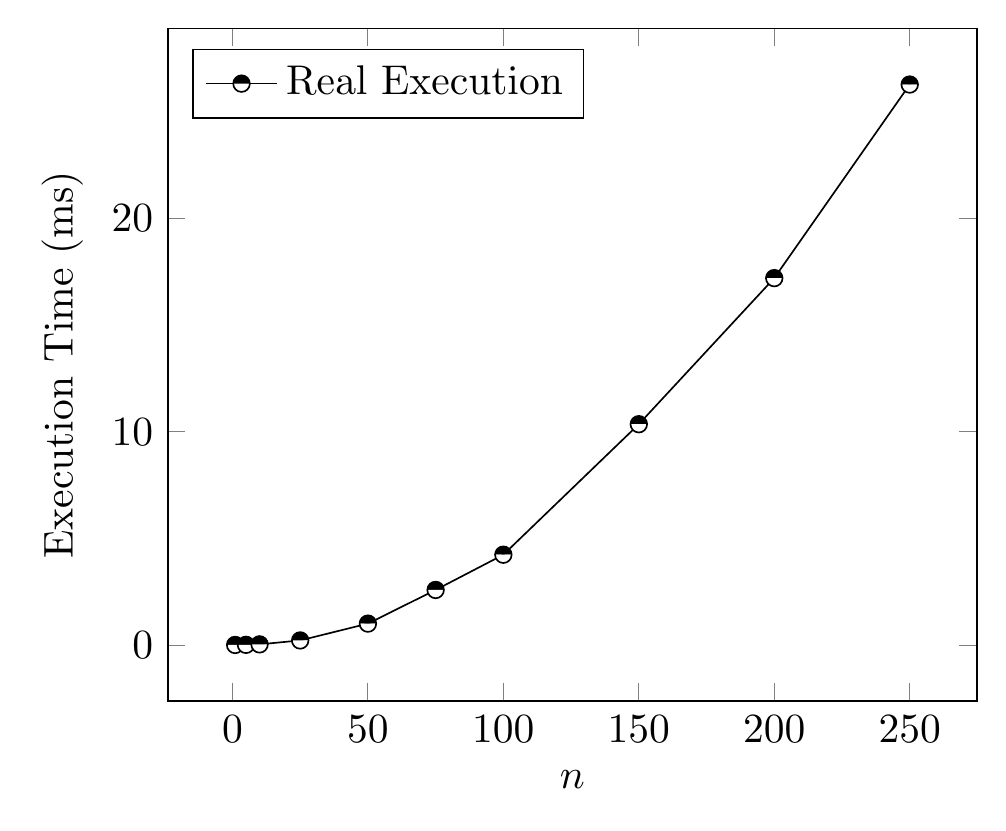
\begin{tikzpicture}[scale = 1.5]
\begin{axis}[domain=0:250, samples=10,grid=minor,
    restrict y to domain=0:30,xlabel=$n$,ylabel=Execution Time (ms), 
    legend pos=north west]
\addplot[
    color=black,
    mark=halfcircle*,
    ]
    coordinates {(1, 0.004768372)
 (5,0.010967255)
 (10,0.031948090)
 (25,0.216007233)
 (50,1.003980637)
 (75,2.583026886)
 (100,4.234075546)
 (150,10.351896286)
 (200,17.199993134)
 (250,26.273965836)
 };
\legend{Real Execution}
\end{axis}
\end{tikzpicture}
\end{center}


\begin{center}
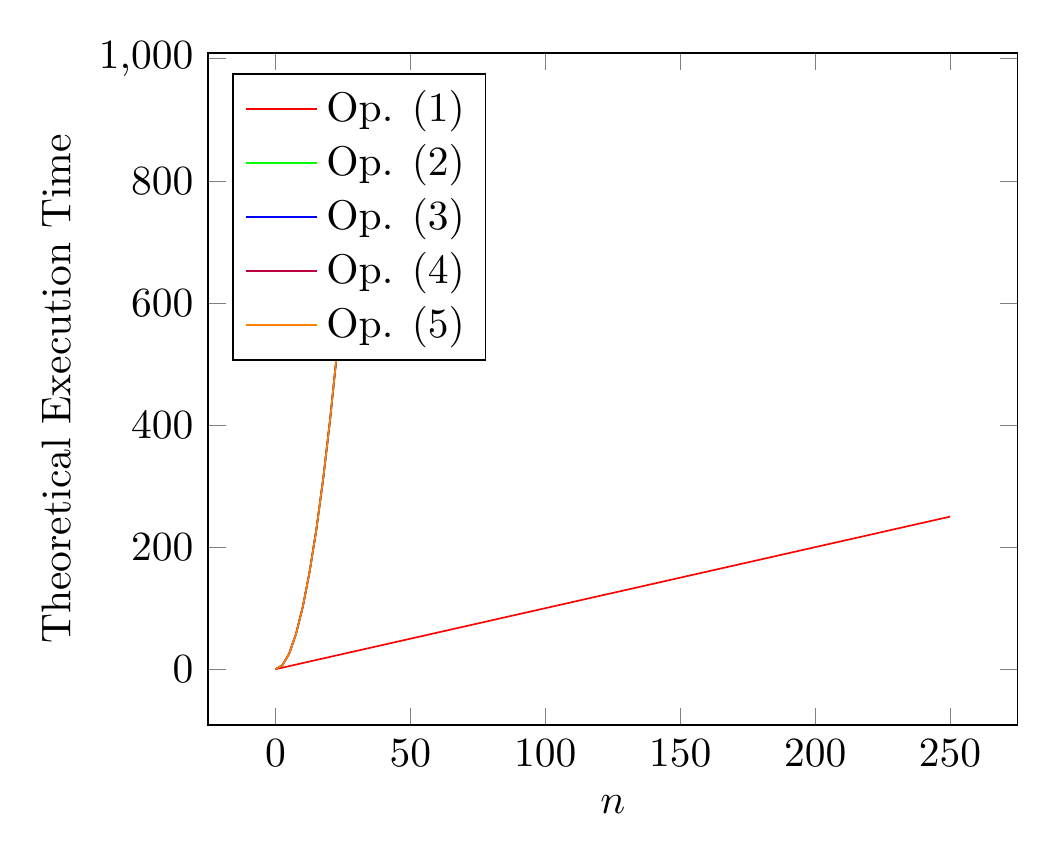
\begin{tikzpicture}[scale = 1.5]
\begin{axis}[domain=0:250, samples=100,grid=minor,
    restrict y to domain=0:1000,xlabel=$n$,ylabel=Theoretical Execution Time, 
    legend pos=north west,
    ]

\addplot [color=red]{x};
\addlegendentry{Op. (1)}

\addplot [color=green]{x^2};
\addlegendentry{Op. (2)}

\addplot [color=blue]{x^2};
\addlegendentry{Op. (3)}

\addplot [color=purple]{x^2};
\addlegendentry{Op. (4)}

\addplot [color=orange]{x^2};
\addlegendentry{Op. (5)}


\end{axis}
\end{tikzpicture}
\end{center}


\subsection{Worst Case}
\begin{center}
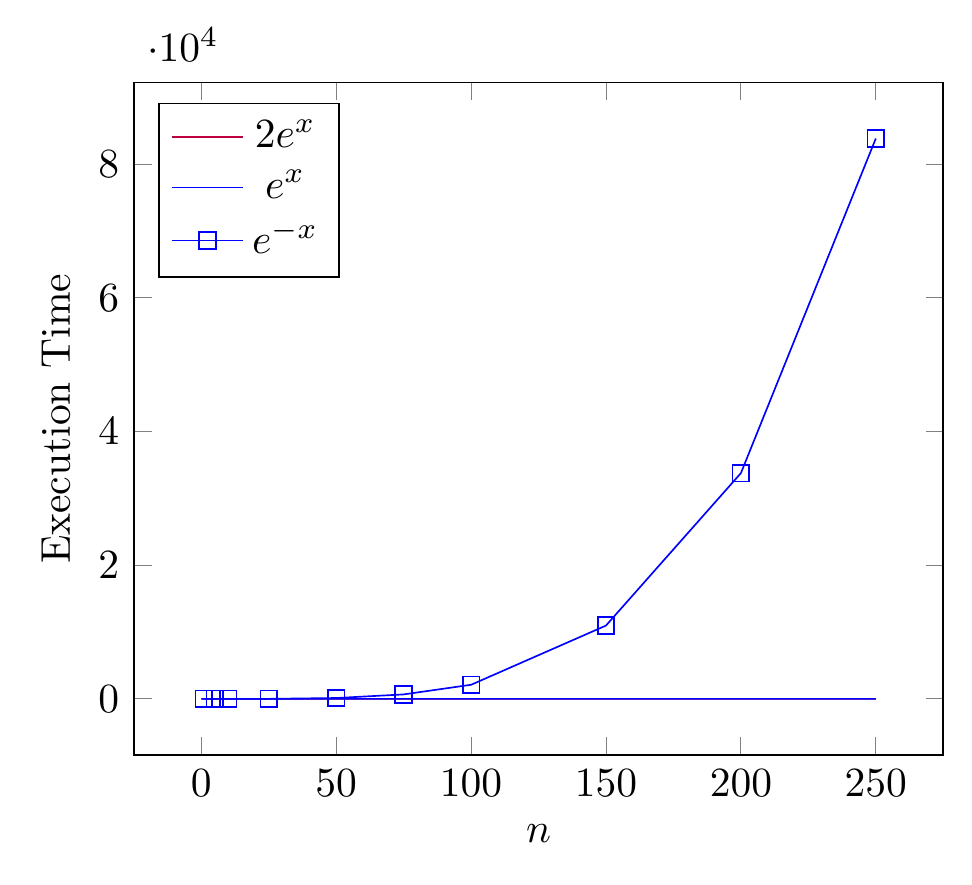
\begin{tikzpicture}[scale = 1.5]
\begin{axis}[domain=0:250, samples=10,grid=minor,
    restrict y to domain=0:85000,xlabel=$n$,ylabel=Execution Time, 
    legend pos=north west]
\addplot [color=purple] {exp(-x)}; 
\addplot [color=blue]   {2*exp(-x)};
\addplot[
    color=blue,
    mark=square,
    ]
    coordinates {(1,0.002861023)
 (5,0.026941299)
 (10,0.254154205)
 (25,8.384943008)
 (50,133.820772171)
 (75,671.449661255)
 (100,2112.159013748)
 (150,10967.132091522)
 (200,33765.886068344)
 (250,83805.630207062)
 };
 
\legend{$2e^x$, $e^x$, $e^{-x}$, $2e^{-x}$}
\end{axis}
\end{tikzpicture}
\end{center}


\subsection{Average Case}
\begin{center}
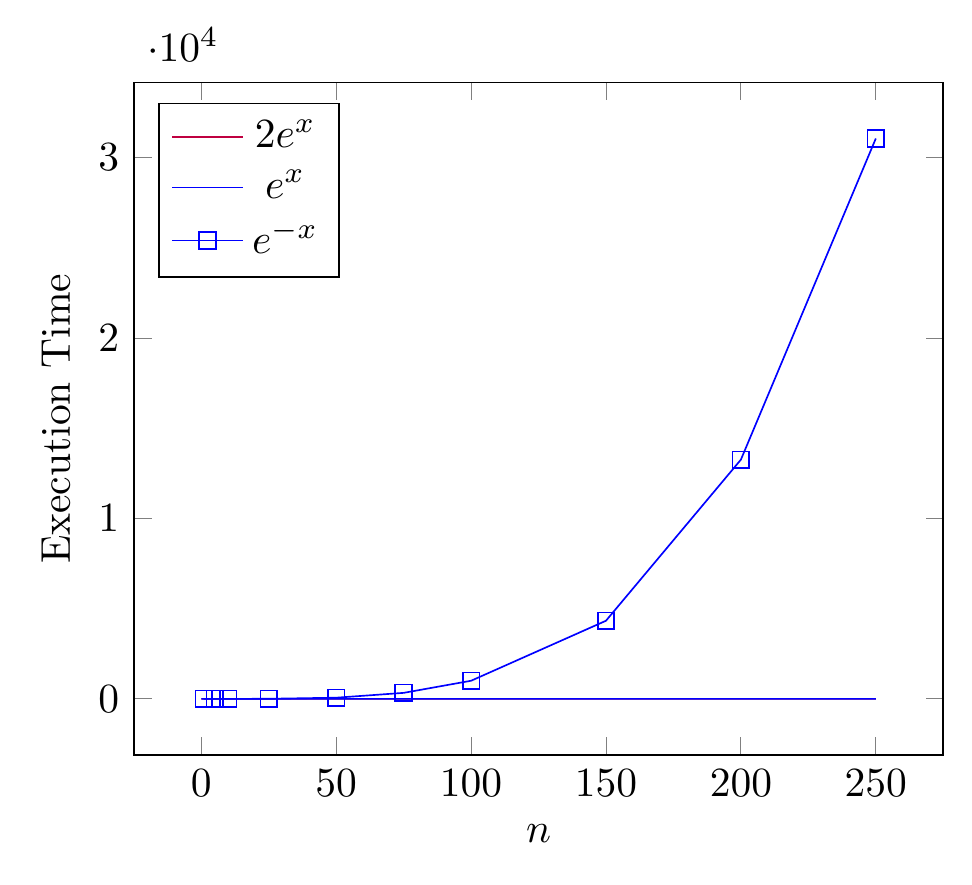
\begin{tikzpicture}[scale = 1.5]
\begin{axis}[domain=0:250, samples=10,grid=minor,
    restrict y to domain=0:32000,xlabel=$n$,ylabel=Execution Time, 
    legend pos=north west]
\addplot [color=purple] {exp(-x)}; 
\addplot [color=blue]   {2*exp(-x)};
\addplot[
    color=blue,
    mark=square,
    ]
    coordinates {(1,0.006437302)
 (5,0.029881795)
 (10,0.379641851)
 (25,7.709662120)
 (50,66.747744878)
 (75,334.980964661)
 (100,1006.102959315)
 (150,4331.564426422)
 (200,13257.391373316)
 (250,31049.947659175)
 };
 
\legend{$2e^x$, $e^x$, $e^{-x}$, $2e^{-x}$}
\end{axis}
\end{tikzpicture}
\end{center}

\end{document}
